\section{Usage}
\label{sec:usage}

Before examining the conversion in detail, this section presents md2h5p from the user's perspective:
Markdown files are converted into an Interactive Book package, accompanied by conversion warnings.

md2h5p can be used in two ways.
As a command-line program, it converts a folder on the
local machine or a public Git repository.
Alternatively, it can run as a web application that accepts a
repository URL or uploaded files in the browser.

\paragraph{Command Line.}
A local conversion is one command that names the folder holding the
chapters:

\begin{lstlisting}
md2h5p convert --folder notes/
\end{lstlisting}

The folder is expected to hold one Markdown file per chapter, in the order given by a leading number
in the file name (\code{1\_intro.md}, \code{2\_setup.md}, \ldots), together with the images those
files reference.
The package is written to the directory the command was run from, named after the
folder unless overridden by \code{--output}.
The folder name also serves as the book's title if no \code{--title} is specified.
To convert a repository instead, \code{--repo} takes its URL
and, if the chapters are not at the root, \code{--subfolder} takes the path inside it.
A further option,
\code{--merge-with}, takes a package that was previously generated and has since been edited in the H5P editor.
The conversion then inserts what was added there into the new package.
Warnings are printed to the console after the conversion.

\begin{figure}[H]
	\centering
	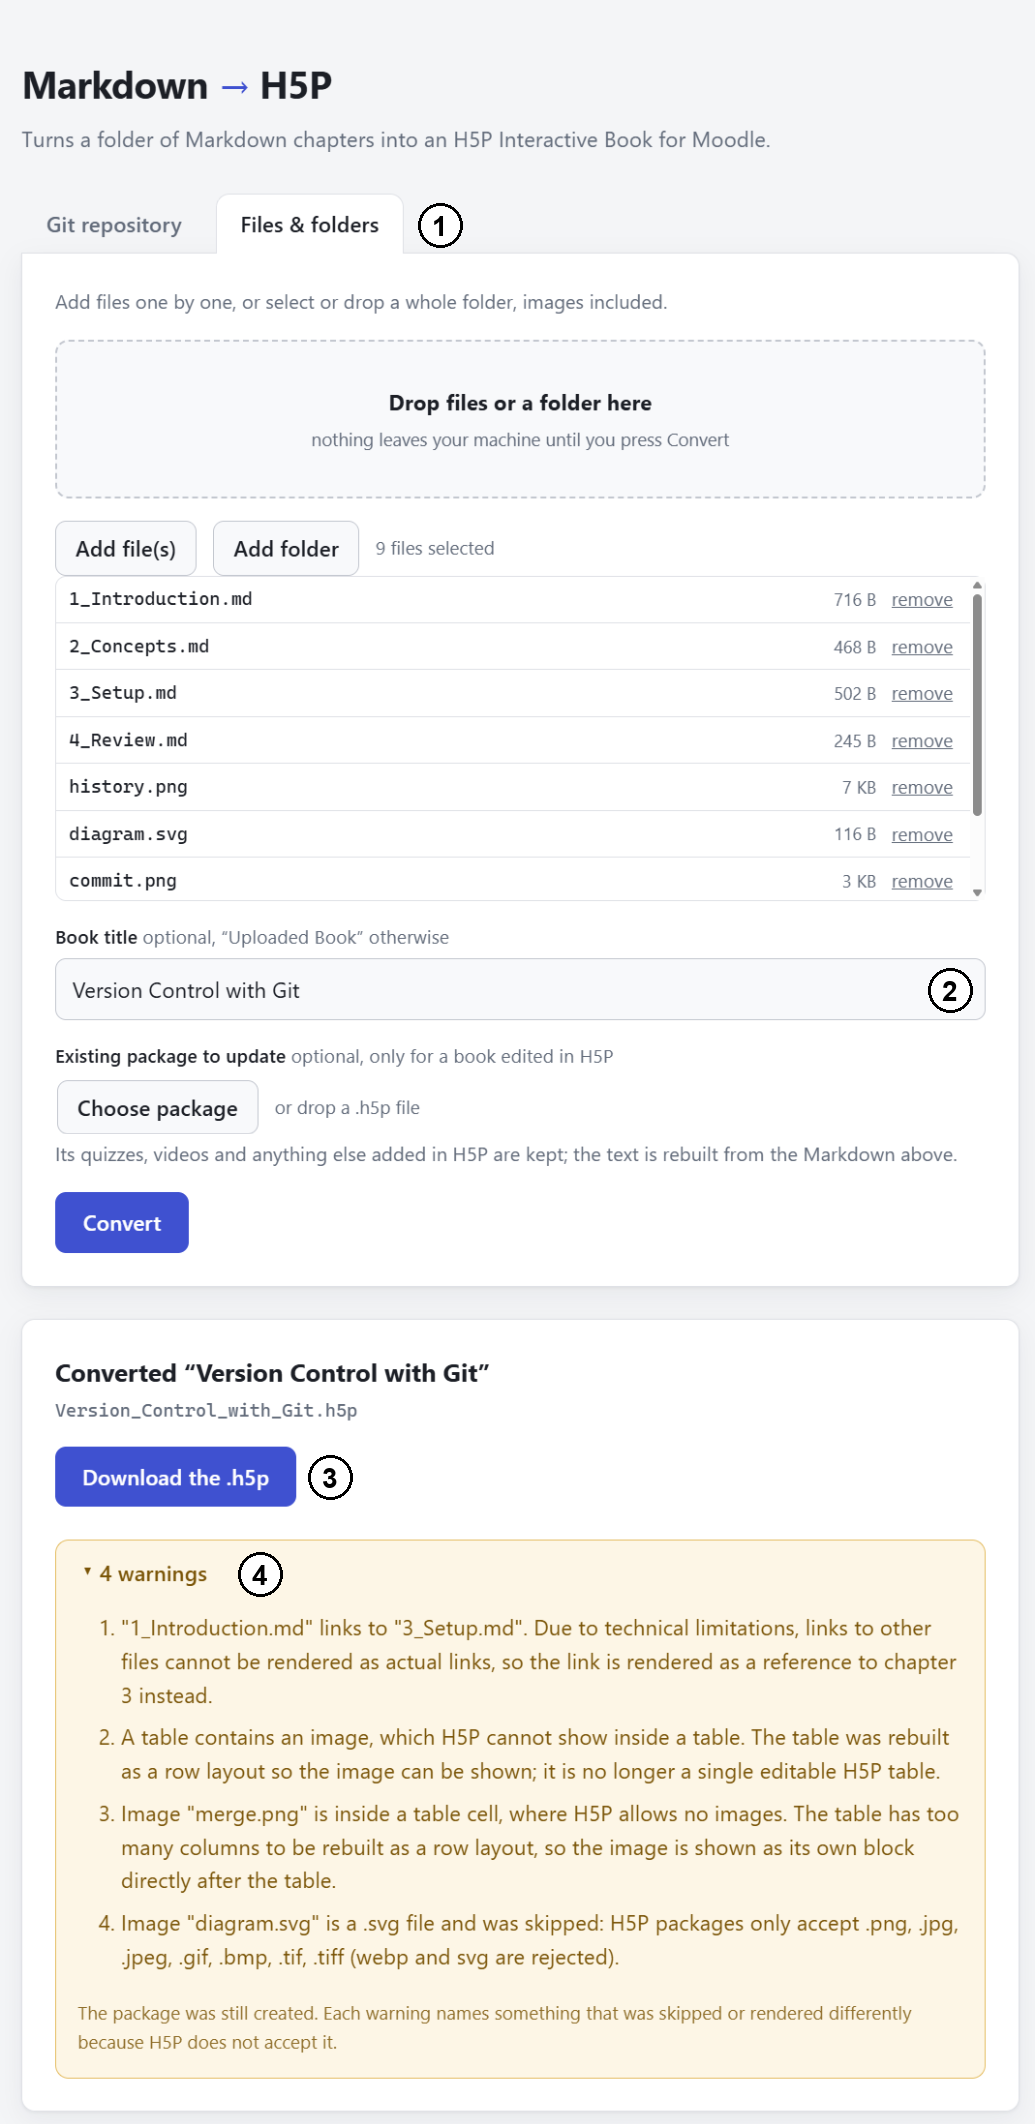
\includegraphics[width=0.68\columnwidth]{figures/screenshots/usage-web}
	\caption[The web interface after a conversion]{\label{fig:usage_web}The web interface after a conversion.
	The warnings \circled{4}
		are part of the result and appear beside the download \circled{3}.}
\end{figure}

\paragraph{Web Interface.}
The server is started with \code{md2h5p serve} and shows one page.
It has two tabs, one for converting a repository and one for uploaded files.
The web UI offers the same configuration options as the CLI: an optional title field, a subfolder field, and a file input for an existing \code{.h5p} package to merge into the new package.
The user starts the conversion by pressing \emph{Convert}.
Once the server has finished, the page shows a result panel with the title, the file name, a download
button, and the list of warnings.
\autoref{fig:usage_web} shows the page after a conversion.

\begin{figure}[H]
	\centering
	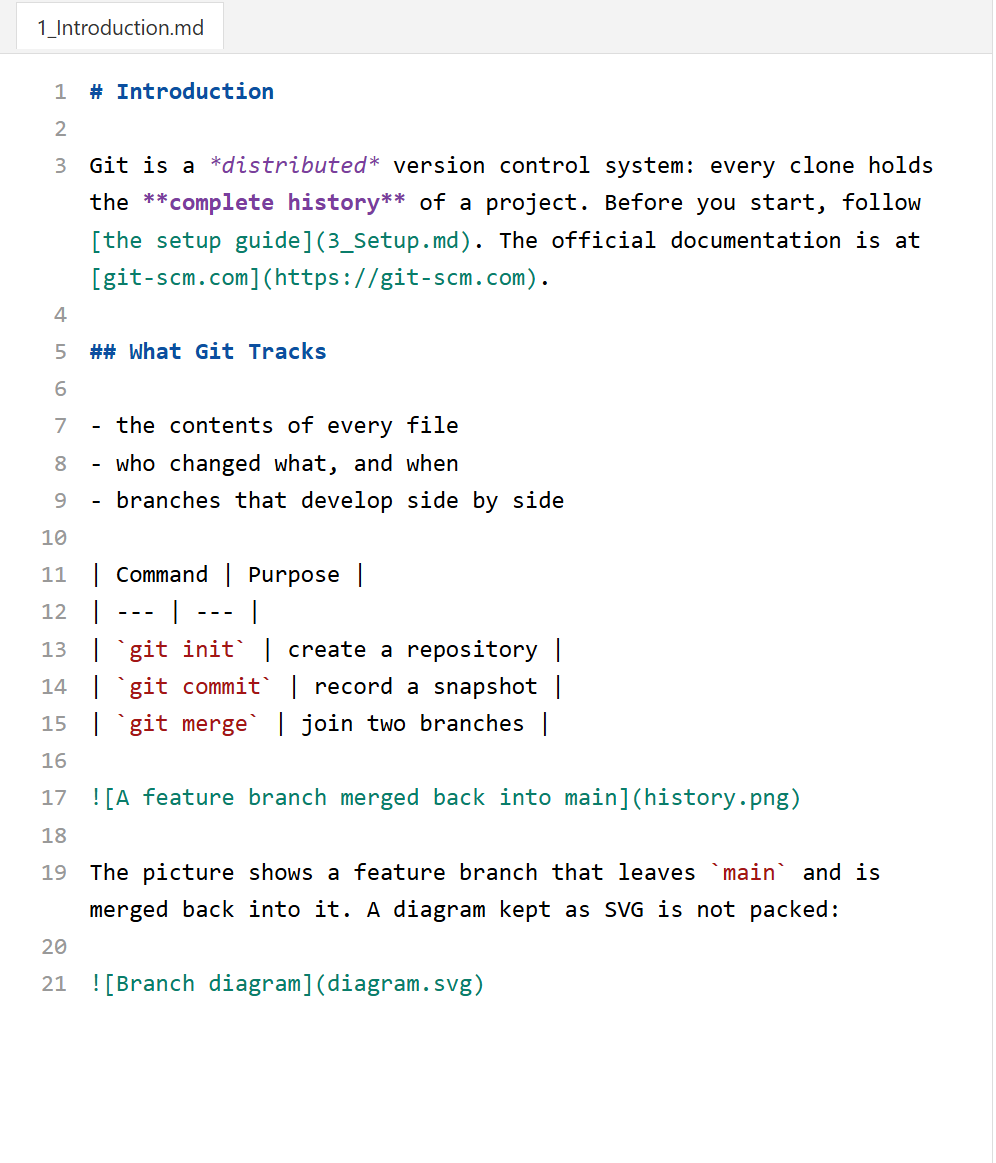
\includegraphics[width=0.485\columnwidth]{figures/screenshots/usage-result-editor}\hfill
	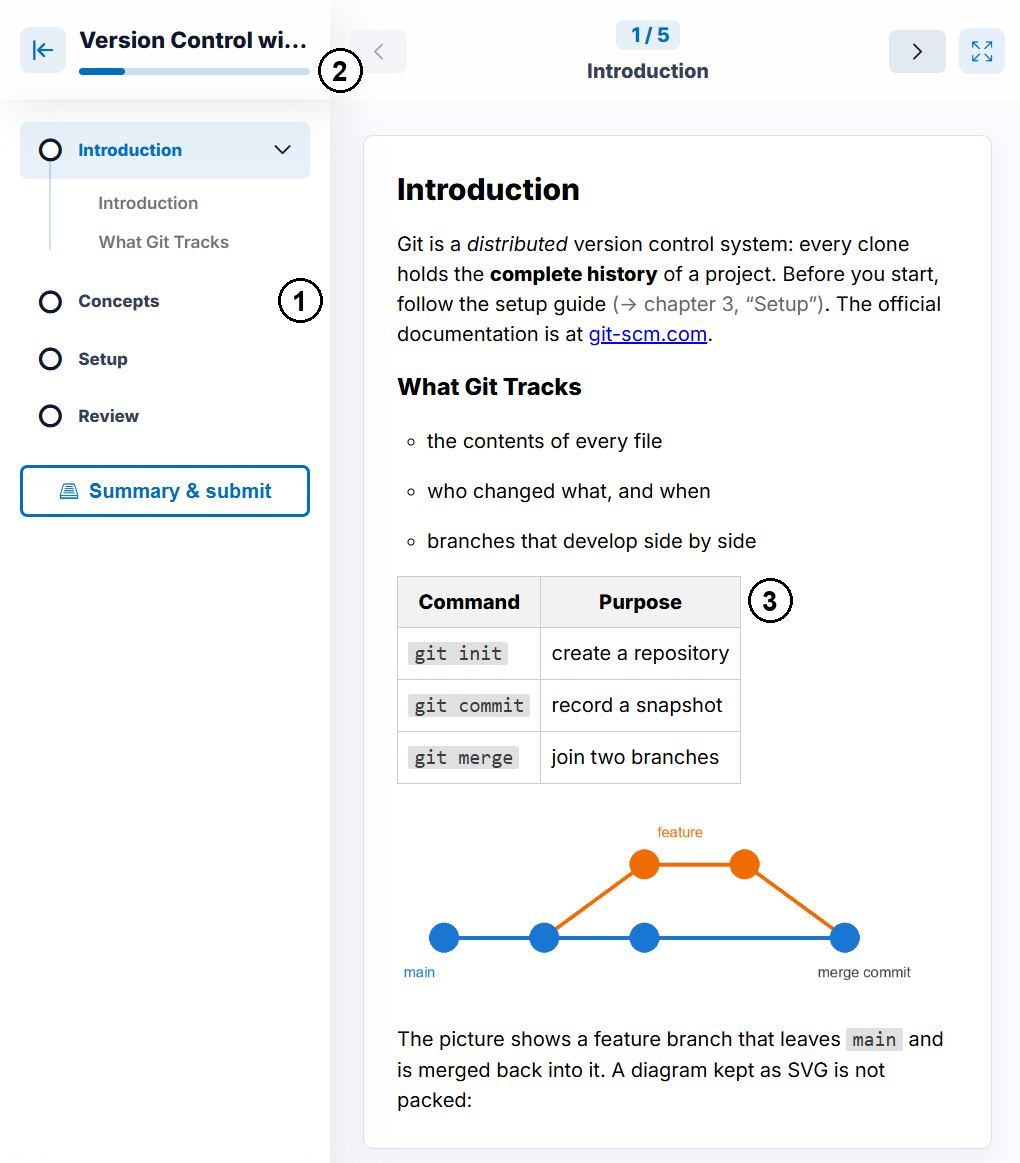
\includegraphics[width=0.485\columnwidth]{figures/screenshots/usage-result-moodle}
	\caption[A chapter in Markdown and in Moodle]{\label{fig:usage_result}A chapter as written in Markdown and as read in Moodle.
	Every
		file has become a chapter with an entry in the sidebar \circled{1}, the book tracks progress
		\circled{2}, and the table \circled{3} carries its borders although the target has no
		stylesheet for it.}
\end{figure}

\paragraph{The Result.}
\autoref{fig:usage_result} shows a chapter as it was written
and as it is read in Moodle.
On the left is the Markdown file in an editor; on the right, the same chapter in
Moodle.
Each file has become a chapter with the file's first heading as its title. The
chapters appear in the sidebar as a table of contents, with every heading of a chapter listed
below it.
The book also keeps a progress indicator across chapters.
To move between them, the reader uses the sidebar or the next and previous buttons.
The text, its formatting, the table, and the image on
the right are what the Markdown specified, rendered in the form the platform accepts.
